\documentclass[a4paper,12pt]{article}
\usepackage{color}
\usepackage{graphicx}
\usepackage{subfig}
\usepackage{listings}
\usepackage{movie15}
\usepackage{hyperref}

\definecolor{dkgreen}{rgb}{0,0.6,0}
\definecolor{gray}{rgb}{0.5,0.5,0.5}
\definecolor{mauve}{rgb}{0.58,0,0.82}

\begin{document}

\title{CSC190 Notes}
\author{Aman Bhargva}
\date{January-April 2019}
\maketitle

\tableofcontents

\section{Introduction and Course Information}

\section{Efficiency and Complexity}
There are two things that effect efficiency of a computer algorithm.
\begin{itemize}
\item Space Complexity = cost in terms of memory
\item Time Complexity = cost in terms of steps
\end{itemize}

\section{Ideal vs. Real Computers}
\begin{tabular}{l|l}
Ideal & Real \\
\hline
Automaton + Workbook & Microprocessor + Memory \\
Mathematical Algorithms & Programs (Sea of Functions) \\
Abstract Data Types & Data Structure 
\end{tabular}

\texttt{Note: ADTs are Abstract Data Types}

\section{List ADT implementation in C}
\begin{itemize}
\item An array with length L and end index 'end'
\end{itemize}

\section{Stacks and Queues}
\subsection{Stacks}
\begin{itemize}
\item First in, last out
\item push and pop
\end{itemize}
\subsection{Queues}
\begin{itemize}
\item First in, first out
\item enqueue, dequeue
\end{itemize}

\section{Trees}
\subsection{Types of Traversal:}
\subsubsection{Level Order Traversal: }
In which you read (1) right to left (2) top to bottom.
\subsubsection{Breadth Order Traversal: }
In which you put stuff on the same level of the tree at the same indentation level, and the children of nodes are indented underneath it.

\subsection{Binary Trees: }
\subsection{Mathai's Weird Definition for Binary Trees <==> Normal Trees}
The rule: The first child of a node goes as the left child in the binary tree. All of its siblings are added as RIGHT children of that first child. Etc.
\subsection{Binary Search Trees: }
Think about the binary search algorithm. The rule is simple: Start with the first node. If the thing you want to add is greater than that node, you add it to the RIGHT child tree. Otherwise, you add it to the LEFT child tree. The rule is recursive and super elegant.
\subsubsection{Advantages/Disadvantages of Binary Search Trees: }
\begin{enumerate}
\item Advantage: Will (generally) change search from O(n) to O(log(n)) because you only need to visit every LEVEL instead of every NODE (\#levels = log(\#nodes))
\item Disadvantage: If it's not a balanced tree, you could end up with a BST that has \#levels = \#nodes
\end{enumerate}

\subsection{Self-Balancing BST's: }
The general way we balance binary search trees is with \textbf{rotations}
\paragraph{Level of imbalance: } calculated as nR (number of levels on the right side of the node) minus nL.
\paragraph{Printing Binary Trees in Order: } When you print the left subtree first, then the node, then the right subtree (recursively)
\subsubsection{Types of Rotation: }
\begin{enumerate}
\item Left
\item Right
\item Major Left / Minor Right
\item Major Right / Minor Left
\end{enumerate}

\subsubsection{Right Rotation: }
The left child becomes the head. The left child's parent (the root) becomes the right child, and the left child of the left child becomes maintains its relationship with the left child of the root. The original left child's RIGHT child becomes the left child of the original root. 
\paragraph{When to do this? } whenever nL - nR $\geq$ 2...?

\subsubsection{Left Rotation: }
The right child becomes the head. The right child's parent (the root) becomes the left child, and the right vhild of the right child maintains its relationship with the right child of the original root. The original right child's LEFT child becomes the right child of the original root. 

\subsubsection{Major Right / Minor Left: }
\paragraph{When to do this: } Whenever the balance on the root and the balance on a subtree is opposite, and the absolute balance of the root is greater than or equal to 2. Tl;dr: You want the subtrees to have the same SIGN of balance as the root node before you do big switches. Condition for doing compelex switches is: balance (root) >=2, sign balance (sub-node) doesn't equal the sign balance (root node)

\subsubsection{Summary of Tree Rotations: }
\begin{enumerate}
\item For easy, child-free lines to the right and left (root balance = +-2, child banace = +-1 with same sign), use the corresponding rotation to make them triangle trees.
\item For bent ones with root balance = +-2 and child balance +-1 of opposite sign), use minor rotation to get back to case 1 and do a major rotation on the root. 
\end{enumerate}

\begin{figure}[h]
\centering
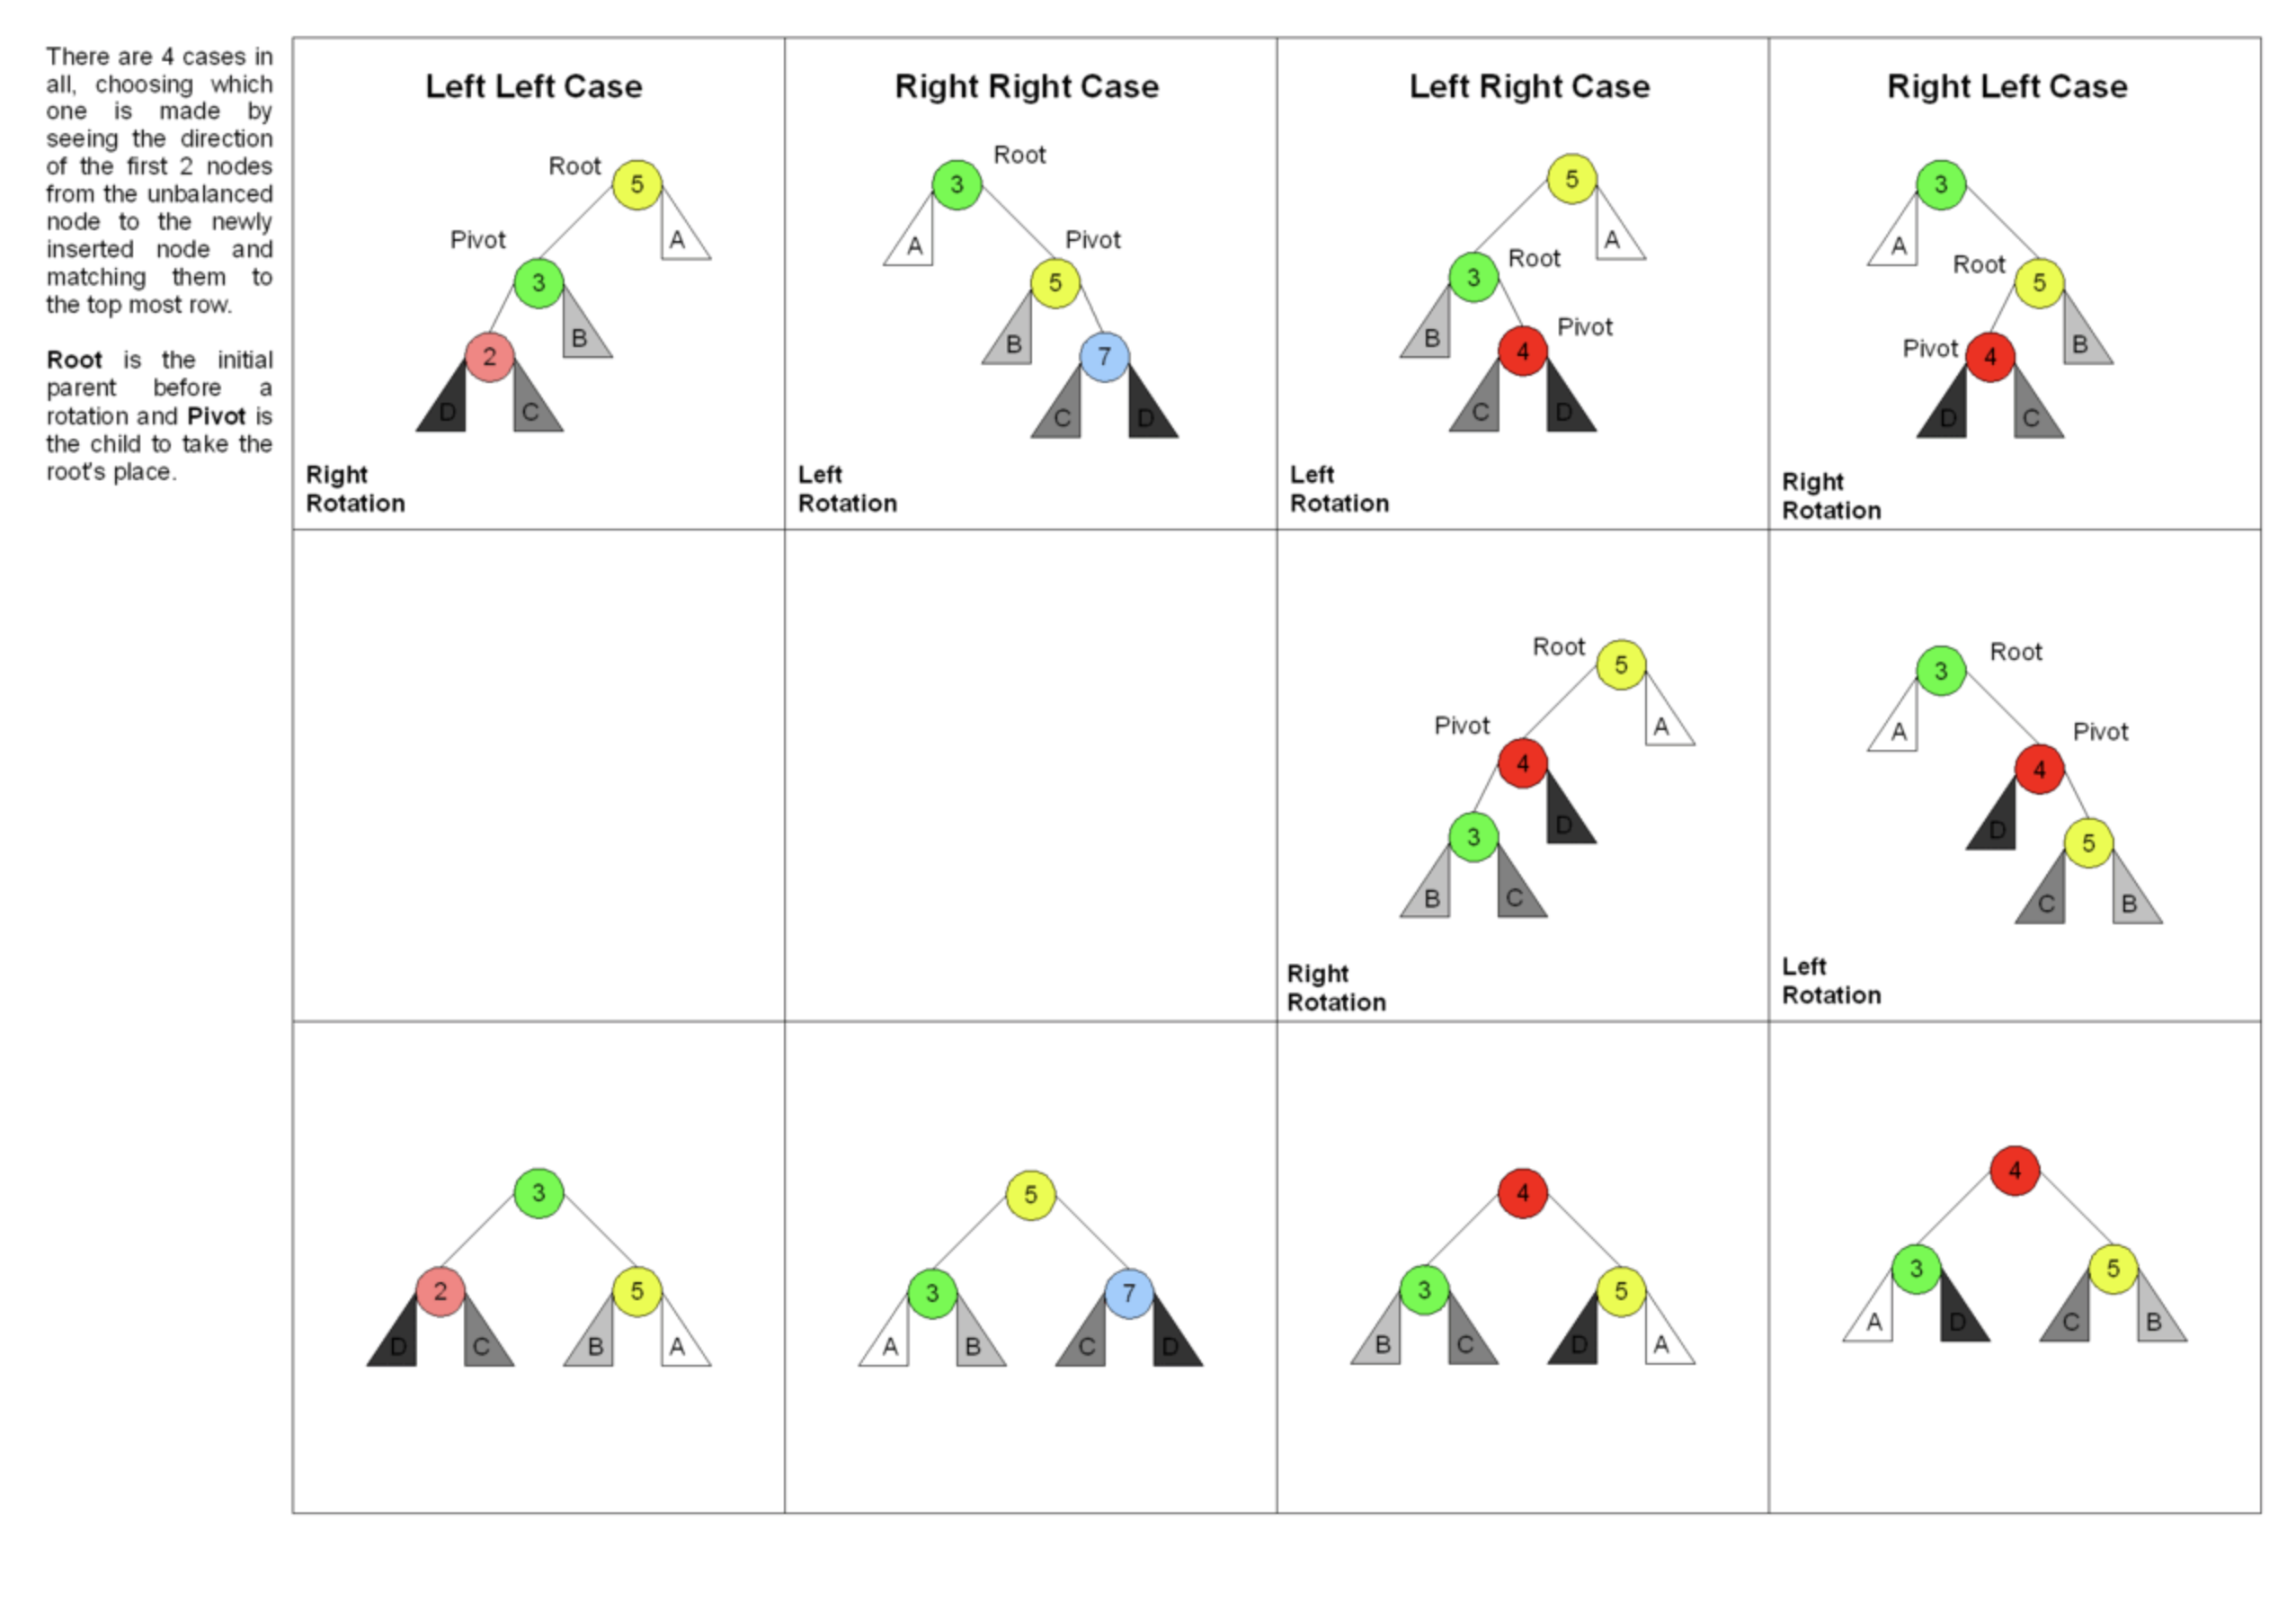
\includegraphics[width=1\textwidth]{media/tree-rotation-summary.png}
\caption{Summary of All Rotation Types}
\label{Tree Rotation Summary}
\end{figure}


\begin{figure}%
    \centering
    \subfloat[label 1]{{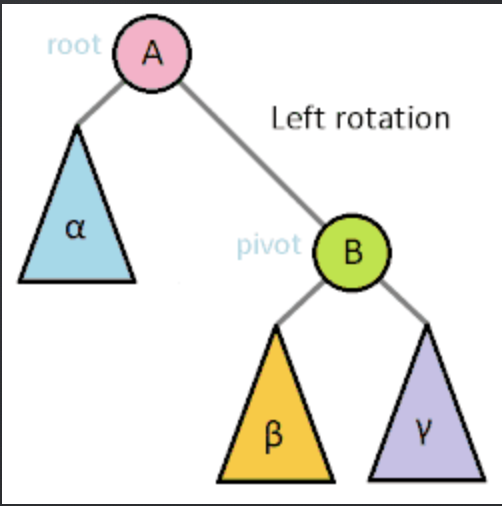
\includegraphics[width=5cm]{media/left-rotation-1.png} }}%
    \qquad
    \subfloat[label 2]{{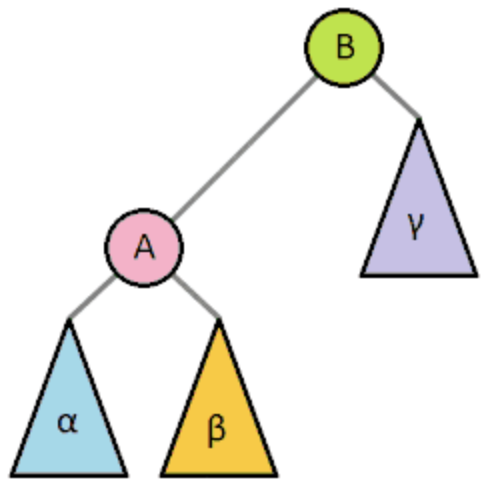
\includegraphics[width=5cm]{media/left-rotation-2.png} }}%
    \caption{Visual Representation of a Left Rotation}%
    \label{fig:example}%
\end{figure}


\begin{figure}%
    \centering
    \subfloat[label 1]{{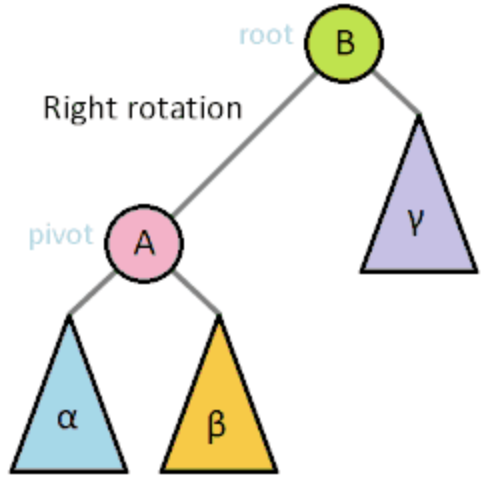
\includegraphics[width=5cm]{media/right-rotation-1.png} }}%
    \qquad
    \subfloat[label 2]{{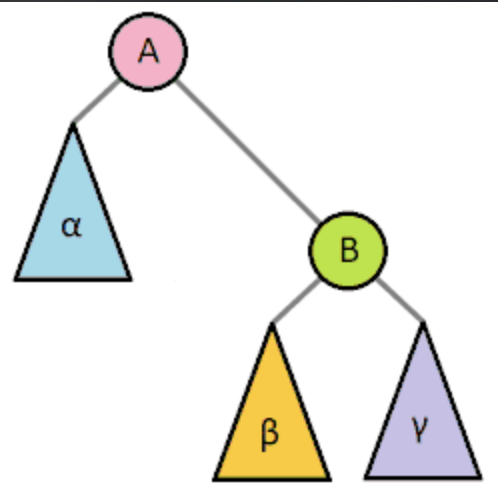
\includegraphics[width=5cm]{media/right-rotation-2.png} }}%
    \caption{Visual Representation of a Right Rotation}%
    \label{fig:example}%
\end{figure}







\end{document}
